\subsection{Implementation details}

\textbf{Models. }In this work, we experimented with four baselines, two CNN-based and two transformer-based backbones. We adopted a ResNet-50 model, along with an application-oriented, embedded vision-based model MobileNetV3-Large (referred to as MobileNetV3). For ResNet, we used the recent ResNetV2-50x1 model (referring further as ResNet50), where x1 denotes the factor by which every hidden layer is widened. Saved checkpoint models for ResNet50 and MobilenetV3 were obtained from \cite{kolesnikov2020big} and \cite{rw2019timm}, respectively. For transformers, we used two SOTA models, namely ViT (B16) and Swin-Transformer, the base variant. These choices were dictated by the fact that these models have achieved SOTA results on several visual perception tasks (classification, object detection, etc.). We used the standard ImageNet21k weights publicly available for initializing our models.    










\textbf{Datasets. }For benchmarking the coreset selection methods, we experiment on four popular datasets. 


\textit{CIFAR10. } CIFAR10 \citep{krizhevsky2009learning} dataset contains 50000 images with 10 classes. We used  as the input to the models in our experiments. We chose this dataset due to its small size and to see the performance of Transformers when trained with small coreset sizes.

\textit{TinyImageNet. } TinyImageNet \citep{wu2017tiny} is a subset of ImageNet21k containing a total of 100k images with 200 classes. This dataset has been created as a smaller, but very good representative of the original Imagenet \cite{russakovsky2015imagenet}. Thus, we use it to show a comparison study of coresets with different backbones close to the ImageNet. 

\textit{APTOS-2019.} APTOS 2019 \citep{aptos2019-blindness-detection}, is medical dataset related to blindness detection. The dataset contains 5 classes, with classification labels ranging from 0 to 4, showing the severity level. In total, APTOS \citep{aptos2019-blindness-detection}, contains 3662 fundus images. This dataset is a good example of non-natural images, and we expect that strong priors learnt on ImageNet21k might not adapt well to this domain.


\textit{UltraMNIST. }This dataset \citep{ultamnist2022} is designed primarily to assess the capability of models to capture semantic coherency in large images. We use  variants of the original dataset. Each sample of UltraMNIST comprises 3-5 MNIST digits of varying scales, and the sum of these digits can vary from 0 to 27, also defining the class labels 0-27. Note that each label in the dataset can be formed with different combinations of the digits, with some classes having very less combinations, while some can be formed by a large number of combinations. Thus, the complexity of the distribution of every class is different, and this makes UltraMNIST an interesting dataset for coreset selection study. For more details related to the dataset, see \cite{ultamnist2022}.




\textbf{Configuration of hyperparameters. } We used the hyperparameters taken from the extensive study by Steiner et al.~\citep{steiner2021train}: SGD momentum optimizer, cosine decay schedule, no weight decay, gradient clipping at global norm 1 and 224×224 image resolution for CIFAR10, Tiny-Imagenet, APTOS-2019, and 512x512 for UltraMNIST.
For the sake of fair comparison, all other hyperparameters are similar across all the backbones and datasets used in this study.








\subsection{Results}
\begin{figure}
\centering
\begin{subfigure}{1\linewidth}  
\centering
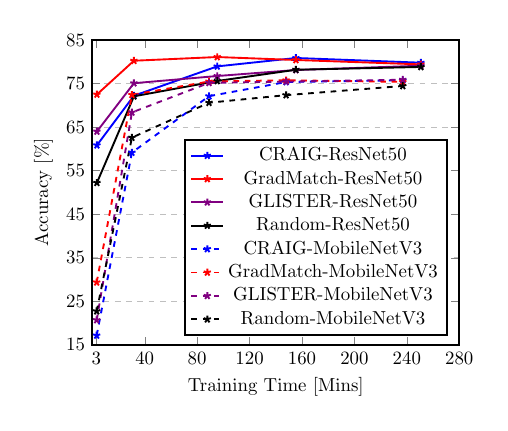
\begin{tikzpicture}[scale=0.68]
   \begin{axis}[ xlabel={Training Time [Mins]},
    ylabel={Accuracy [\%]},
   xmin=0, xmax=280,
    ymin=15, ymax=85,
    xtick={3, 40, 80, 120, 160, 200, 240, 280},
    ytick={15, 25, 35, 45, 55, 65, 75, 85},
    legend pos=south east,
    ymajorgrids=true,
    grid style=dashed,
    line width=1pt,
    ]
 \addplot[
    color=blue,
    mark=star,
    ]
    coordinates {
    (3.53,60.83)
    (31.78, 72.21)
    (95.35,78.94)
    (155.38,80.87)
    (250.73,79.79)};
    \addlegendentry{CRAIG-ResNet50}

\addplot[
    color=red,
    mark=star,
    ]
    coordinates {
    (3.53, 72.49)
    (31.78, 80.24)
    (95.35, 81.09)
    (155.38, 80.41)
    (250.73, 79.40)};
    \addlegendentry{GradMatch-ResNet50}

\addplot[
    color=violet,
    mark=star,
    ]
    coordinates {
    (3.53, 63.99)
    (31.78, 75.08)
    (95.35, 76.73)
    (155.38, 78.11)
    (250.73, 79.09)};
    \addlegendentry{GLISTER-ResNet50}

    \addplot[
        color=black,
        mark=star,
        ]
        coordinates {
        (3.53, 52.21)
        (31.78, 72.07)
        (95.35, 75.59)
        (155.38, 78.17)
        (250.73, 78.81)
        };
        \addlegendentry{Random-ResNet50}

    \addplot[
    color=blue,
    mark=star,
    dashed
    ]
    coordinates {
    (3.36,17.15)
    (30.24, 59.15)
    (89.05,72.10)
    (147.87,75.35)
    (236.92,75.76)};
    \addlegendentry{CRAIG-MobileNetV3}

\addplot[
    color=red,
    mark=star,
    dashed
    ]
    coordinates {
    (3.36, 29.35)
    (30.24, 72.42)
    (89.05, 75.47)
    (147.87, 75.75)
    (236.92, 75.39)};
    \addlegendentry{GradMatch-MobileNetV3}

\addplot[
    color=violet,
    mark=star,
    dashed
    ]
    coordinates {
    (3.36, 20.68)
    (30.24, 68.37)
    (89.05, 75.15)
    (147.87, 75.45)
    (236.92, 75.87)};
    \addlegendentry{GLISTER-MobileNetV3}
    \addplot[
        color=black,
        mark=star,
        dashed
        ]
        coordinates {
        (3.36, 22.72)
        (30.24, 62.58)
        (89.05, 70.60)
        (147.87, 72.34)
        (236.92, 74.44)
        };
        \addlegendentry{Random-MobileNetV3}
    \end{axis}
    \end{tikzpicture}~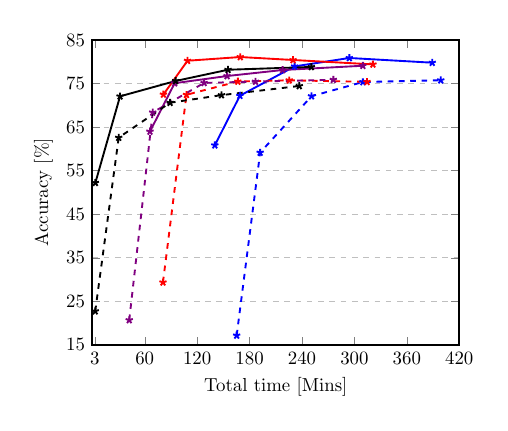
\begin{tikzpicture}[ scale=0.68]
    \begin{axis}[ xlabel={Total time [Mins]},
    ylabel={Accuracy [\%]},
    xmin=0, xmax=420,
    ymin=15, ymax=85,
    xtick={3, 60, 120, 180, 240, 300, 360, 420},
    ytick={15, 25, 35, 45, 55, 65, 75, 85},
ymajorgrids=true,
    grid style=dashed,
    line width=1pt,    
    ]
\addplot[
    color=blue,
    mark=star,
    ]
    coordinates {
    (140.30,60.83)
    (168.94, 72.21)
    (231.58,78.94)
    (294.23,80.87)
    (389.09,79.79)};


\addplot[
    color=red,
    mark=star,
    ]
    coordinates {
    (81.42, 72.49)
    (109.02, 80.24)
    (169.40, 81.09)
    (229.79, 80.41)
    (321.22, 79.40)};


\addplot[
    color=violet,
    mark=star,
    ]
    coordinates {
    (66.01, 63.99)
    (94.27, 75.08)
    (154.30, 76.73)
    (217.87, 78.11)
    (309.69, 79.09)};


    \addplot[
        color=black,
        mark=star,
        ]
        coordinates {
        (3.53, 52.21)
        (31.78, 72.07)
        (95.35, 75.59)
        (155.38, 78.17)
        (250.73, 78.81)
        };


    \addplot[
    color=blue,
    mark=star,
    dashed
    ]
    coordinates {
    (165.27,17.15)
    (192.15, 59.15)
    (250.97,72.10)
    (309.78,75.35)
    (398.84,75.76)};


\addplot[
    color=red,
    mark=star,
    dashed
    ]
    coordinates {
    (80.91, 29.35)
    (107.79, 72.42)
    (166.60, 75.47)
    (225.42, 75.75)
    (314.47, 75.39)};


\addplot[
    color=violet,
    mark=star,
    dashed
    ]
    coordinates {
    (42.30, 20.68)
    (69.18, 68.37)
    (127.99, 75.15)
    (186.81, 75.45)
    (275.87, 75.87)};


    
    

\addplot[
    color=black,
    mark=star,
    dashed
    ]
    coordinates {
    (3.36, 22.72)
    (30.24, 62.58)
    (89.05, 70.60)
    (147.87, 72.34)
    (236.92, 74.44)
    };
\end{axis}
    \end{tikzpicture}\vspace{-0.2em}
\caption{CNN (Solid - ResNet50; Dashed - MobileNetV3)}
\label{fig;sub-comp-corecnn}
\end{subfigure}









\begin{subfigure}{1\linewidth}   
\centering
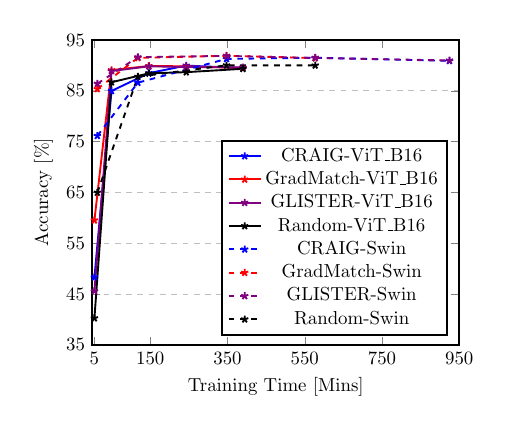
\begin{tikzpicture}[scale=0.68]
   \begin{axis}[ xlabel={Training Time [Mins]},
    ylabel={Accuracy [\%]},
   xmin=0, xmax=950,
    ymin=35, ymax=95,
    xtick={5, 150, 350, 550, 750, 950},
    ytick={35, 45, 55, 65, 75, 85, 95},
    legend pos=south east,
    ymajorgrids=true,
    grid style=dashed,
    line width=1pt,
    ]
 \addplot[
    color=blue,
    mark=star,
    ]
    coordinates {
    (5.53,48.30)
    (49.77, 84.97)
    (146.56,88.48)
    (243.35,89.97)
    (389.91,89.46)};
    \addlegendentry{CRAIG-ViT\_B16}

\addplot[
    color=red,
    mark=star,
    ]
    coordinates {
    (5.53,59.51)
    (49.77, 89.07)
    (146.56,89.89)
    (243.35,89.82)
    (389.91,89.50)};
    \addlegendentry{GradMatch-ViT\_B16}

\addplot[
    color=violet,
    mark=star,
    ]
    coordinates {
    (5.53,45.59)
    (49.77, 88.89)
    (146.56,89.82)
    (243.35,89.69)
    (389.91,89.60)};
    \addlegendentry{GLISTER-ViT\_B16}

    \addplot[
        color=black,
        mark=star,
        ]
        coordinates {
        (5.53,40.24)
        (49.77, 86.69)
        (146.56,88.44)
        (243.35,88.67)
        (389.91,89.33)};
        \addlegendentry{Random-ViT\_B16}

    \addplot[
    color=blue,
    mark=star,
    dashed
    ]
    coordinates {
    (13.11, 76.14)
    (118.04, 86.60)
    (347.57, 91.28)
    (577.09, 91.51)
    (924.67, 90.89)
    };
    \addlegendentry{CRAIG-Swin}

\addplot[
    color=red,
    mark=star,
    dashed
    ]
    coordinates {
    (13.11, 85.37)
    (118.04, 91.48)
    (347.57, 91.90)
    (577.09, 91.44)
};
    \addlegendentry{GradMatch-Swin}

\addplot[
    color=violet,
    mark=star,
    dashed
    ]
    coordinates {
    (13.11, 86.41)
    (118.04, 91.63)
    (347.57, 91.87)
    (577.09, 91.47)
    (924.67, 90.97)
    };
    \addlegendentry{GLISTER-Swin}

    
    

    \addplot[
        color=black,
        mark=star,
        dashed
        ]
        coordinates {
        (13.11, 64.97)
        (118.04, 87.77)
        (347.57, 90.02)
        (577.09, 90.00)
};
        \addlegendentry{Random-Swin}
    \end{axis}
    \end{tikzpicture}~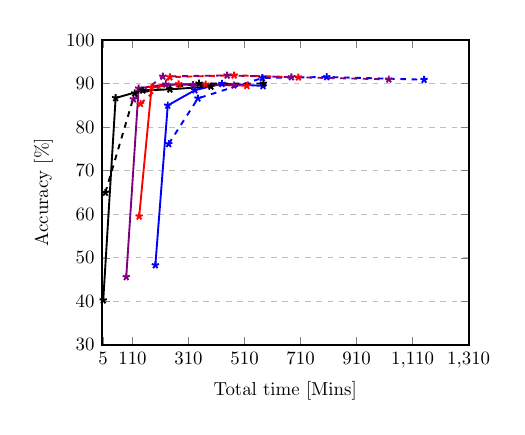
\begin{tikzpicture}[ scale=0.68]
    \begin{axis}[ xlabel={Total time [Mins]},
    ylabel={Accuracy [\%]},
    xmin=0, xmax=1310,
    ymin=30, ymax=100,
    xtick={5, 110, 310, 510, 710, 910, 1110, 1310},
    ytick={30, 40, 50, 60, 70, 80, 90, 100},
ymajorgrids=true,
    grid style=dashed,
    line width=1pt,    
    ]

    \addplot[
    color=blue,
    mark=star,
    ]
    coordinates {
    (191.59,48.30)
    (235.84, 84.97)
    (332.62,88.48)
    (429.41,89.97)
    (575.97,89.46)};


    \addplot[
        color=red,
        mark=star,
        ]
        coordinates {
        (133.82,59.51)
        (178.07, 89.07)
        (274.86,89.89)
        (371.64,89.82)
        (518.21,89.50)};


    \addplot[
        color=violet,
        mark=star,
        ]
        coordinates {
        (87.67,45.59)
        (131.92, 88.89)
        (228.71,89.82)
        (325.49,89.69)
        (472.06,89.60)};


    \addplot[
        color=black,
        mark=star,
        ]
        coordinates {
        (5.53,40.24)
        (49.77, 86.69)
        (146.56,88.44)
        (243.35,88.67)
        (389.91,89.33)};


    \addplot[
        color=blue,
        mark=star,
        dashed
        ]
        coordinates {
        (239.26, 76.14)
        (343.56, 86.60)
        (573.72, 91.28)
        (803.24, 91.51)
        (1150.82, 90.89)
        };


    \addplot[
        color=red,
        mark=star,
        dashed
        ]
        coordinates {
        (138.36, 85.37)
        (243.29, 91.48)
        (472.82, 91.90)
        (702.34, 91.44)
};


    \addplot[
        color=violet,
        mark=star,
        dashed
        ]
        coordinates {
        (113.39, 86.41)
        (218.32, 91.63)
        (447.89, 91.87)
        (677.37, 91.47)
        (1024.94, 90.97)
        };


    
    

    \addplot[
        color=black,
        mark=star,
        dashed
        ]
        coordinates {
        (13.11, 64.97)
        (118.04, 87.77)
        (347.57, 90.02)
        (577.09, 90.00)
};



    \end{axis}
    \end{tikzpicture}\vspace{-0.2em}
\caption{Transformer (Solid - ViT\_B16; Dashed - Swin)}
\label{fig:sub-comp-coretran}
\end{subfigure}
\vspace{-2em}
\caption{Performance scores for various coreset selection methods for different choices of training time as well as total time. Models are pretrained on ImageNet21k and further trained for TinyImageNet classification.}
\label{fig:sub-comp-core}
\end{figure}






%
 We discuss below the results related to the various benchmarking experiments conducted in this paper. 


\textbf{Comparison of coreset selection methods. }To the best of our knowledge, a clear comparison of the recent coreset selection methods in terms of training time does not exist, especially for transformers. We begin with benchmarking our selected models, using 4 coreset selection methods as described above. Fig. \ref{fig:sub-comp-core}, illustrates the performance comparison in terms of training time along with the total time (training + coreset selection). From a practical perspective, the total time needs to be reduced. However, it can be argued that coreset selection can be scaled across multiple CPU threads, thereby making the coreset selection time very small. 


 


For ResNet and MobileNet, except for random selection, GradMatch consistently outperforms other methods. Whereas, for longer training time, CRAIG is only marginally better. For very small coresets, GLISTER is outperformed by even the random selection method. As for the total time, except for GradMatch, all methods get outperformed by random selection (especially, small time budgets), which is counterintuitive and implies that the coreset selection methods are not stable for CNNs at low training time budgets. 

Similar observations are made for transformer models (all training time). For small time budgets, we see that for ViT\_B16 as well as the Swin transformer, random coreset selection performs better than other methods, clearly indicating that a generalizable solution to make models time-efficient through coreset selection is still missing.







\begin{figure}
        \centering
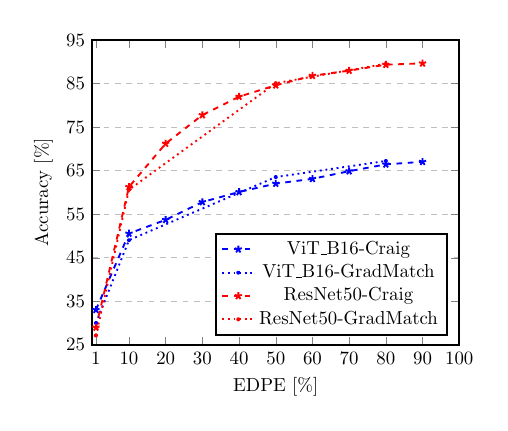
\begin{tikzpicture}[scale=0.68]
   \begin{axis}[ xlabel={EDPE [\%]},
    ylabel={Accuracy [\%]},
    xmin=0, xmax=100,
    ymin=25, ymax=95,
   xtick={1, 10, 20, 30, 40, 50, 60, 70, 80, 90, 100},
    ytick={0, 25, 35, 45, 55, 65, 75, 85, 95},
    legend pos=south east,
    ymajorgrids=true,
    grid style=dashed,
    line width=1pt,
    ]
\addplot[
    color=blue,
    mark=star,
    dashed
    ]
    coordinates {
    (1,33.04)
    (10,50.57)
    (20,53.70)
    (30,57.79)
    (40,60.10)
    (50,62.02)
    (60,63.12)
    (70,64.88)
    (80,66.44)
    (90,67.03)
    };
    \addlegendentry{ViT\_B16-Craig}

\addplot[
    color=blue,
    mark=star,
    dotted
    ]
    coordinates {
    (1,30.00)
    (10,49.04)
    (50,63.53)
    (80,67.22)
};
    \addlegendentry{ViT\_B16-GradMatch}

    \addplot[
    color=red,
    mark=star,
    dashed
    ]
    coordinates {
    (1,28.98)
    (10,61.27)
    (20,71.22)
    (30,77.76)
    (40,81.99)
    (50,84.60)
    (60,86.79)
    (70,87.97)
    (80,89.33)
    (90,89.64)
    };
    \addlegendentry{ResNet50-Craig}

    \addplot[
    color=red,
    mark=star,
    dotted
    ]
    coordinates {
    (1,27.15)
    (10,60.61)
    (50,85.09)
    (80,89.55)
};
    \addlegendentry{ResNet50-GradMatch}
    \end{axis}
    \end{tikzpicture}~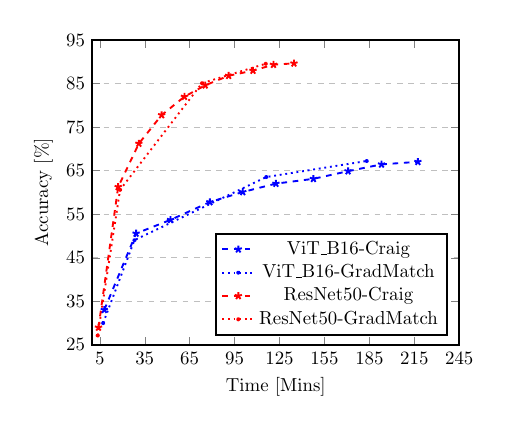
\begin{tikzpicture}[ scale=0.68]
    \begin{axis}[ xlabel={Time [Mins]},
    ylabel={Accuracy [\%]},
    xmin=0, xmax=245,
    ymin=25, ymax=95,
    xtick={5, 35, 65, 95, 125, 155, 185, 215, 245},
    ytick={0, 25, 35, 45, 55, 65, 75, 85, 95},
    legend pos=south east,
    ymajorgrids=true,
    grid style=dashed,
    line width=1pt,    
    ]
\addplot[
    color=blue,
    mark=star,
    dashed
    ]
    coordinates {
    (8.02,33.04)
    (29.24,50.57)
    (52.25,53.70)
    (78.51,57.79)
    (100.47,60.10)
    (122.60,62.02)
    (147.65,63.12)
    (170.78,64.88)
    (193.10,66.44)
    (217.38,67.03)
    };
    \addlegendentry{ViT\_B16-Craig}

\addplot[
    color=blue,
    mark=star,
    dotted
    ]
    coordinates {
    (7.25,30.00)
    (28.16,49.04)
    (116.13,63.53)
    (183.22,67.22)
};
    \addlegendentry{ViT\_B16-GradMatch}

\addplot[
    color=red,
    mark=star,
    dashed
    ]
    coordinates {
    (4.13,28.98)
    (17.29,61.27)
    (31.11,71.22)
    (46.30,77.76)
    (61.54,81.99)
    (75.40,84.60)
    (91.03,86.79)
    (107.29,87.97)
    (120.97,89.33)
    (134.64,89.64)
    };
    \addlegendentry{ResNet50-Craig}

    \addplot[
    color=red,
    mark=star,
    dotted
    ]
    coordinates {
    (3.62,27.15)
    (18.57,60.61)
    (73.27,85.09)
    (115.79,89.55)
};
    \addlegendentry{ResNet50-GradMatch}
    \end{axis}
    \end{tikzpicture}\vspace{-1em}
\caption{Performance comparison between Randomly Initialised \vit and ResNet50 for time, EDPE and performance on CIFAR10, SSI=50.}
\label{fig:rand-train}
\end{figure} 
\textbf{Data subselection under no pretraining. } 
For this study, we conducted experiments on the CIFAR10 dataset, using ResNet50 and VIT-B16 for CRAIG and GradMatch methods. Related results are shown in Fig. \ref{fig:rand-train}. It can be seen that CNN architecture outperforms transformers significantly without pretraining. We argue that it is because transformers are data-hungry and thus are affected severely in the absence of pretraining. More importantly, this also illustrates that without appropriate pretraining, for transformers, coreset selection might become irrelevant. 











\begin{figure}
        \centering
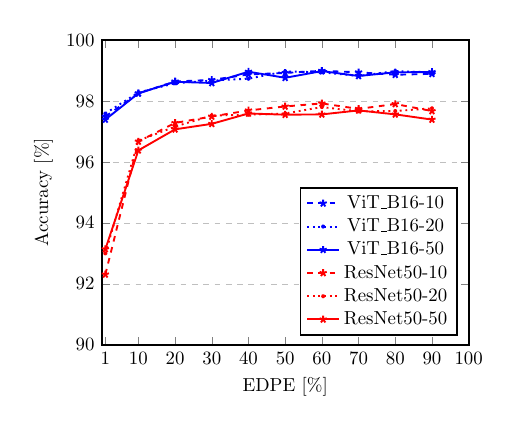
\begin{tikzpicture}[scale=0.68]
   \begin{axis}[ xlabel={EDPE [\%]},
    ylabel={Accuracy [\%]},
    xmin=0, xmax=100,
    ymin=90, ymax=100,
   xtick={1, 10, 20, 30, 40, 50, 60, 70, 80, 90, 100},
    ytick={90, 92, 94, 96, 98, 100},
    legend pos=south east,
    ymajorgrids=true,
    grid style=dashed,
    line width=1pt,
    ]
 \addplot[
    color=blue,
    mark=star,
    dashed
    ]
    coordinates {
    (1,97.49)
    (10,98.25)
    (20,98.64)
    (30,98.69)
    (40,98.87)
    (50,98.92)
    (60,98.99)
    (70,98.94)
    (80,98.86)
    (90,98.89)
    };
    \addlegendentry{ViT\_B16-10}

\addplot[
    color=blue,
   mark=star,
    dotted
    ]
    coordinates {
    (1,97.59)
    (10,98.28)
    (20,98.58)
    (30,98.67)
    (40,98.73)
    (50,98.97)
    (60,98.94)
    (70,98.82)
    (80,98.98)
    (90,98.94)
    };
    \addlegendentry{ViT\_B16-20}

\addplot[
    color=blue,
    mark=star,
    ]
    coordinates {
    (1,97.39)
    (10,98.25)
    (20,98.63)
    (30,98.59)
    (40,98.96)
    (50,98.76)
    (60,98.98)
    (70,98.82)
    (80,98.94)
    (90,98.95)
    };
    \addlegendentry{ViT\_B16-50}

\addplot[
    color=red,
    mark=star,
    dashed
    ]
    coordinates {
    (1,92.31)
    (10,96.67)
    (20,97.28)
    (30,97.49)
    (40,97.69)
    (50,97.82)
    (60,97.92)
    (70,97.74)
    (80,97.90)
    (90,97.67)
    };
    \addlegendentry{ResNet50-10}

\addplot[
    color=red,
    mark=star,
    dotted
    ]
    coordinates {
    (1,93.00)
    (10,96.70)
    (20,97.16)
    (30,97.52)
    (40,97.55)
    (50,97.59)
    (60,97.80)
    (70,97.66)
    (80,97.67)
    (90,97.76)
    };
    \addlegendentry{ResNet50-20}

\addplot[
    color=red,
    mark=star,
    ]
    coordinates {
    (1,93.14)
    (10,96.38)
    (20,97.07)
    (30,97.25)
    (40,97.59)
    (50,97.55)
    (60,97.56)
    (70,97.69)
    (80,97.56)
    (90,97.39)
    };
    \addlegendentry{ResNet50-50}
    \end{axis}
    \end{tikzpicture}~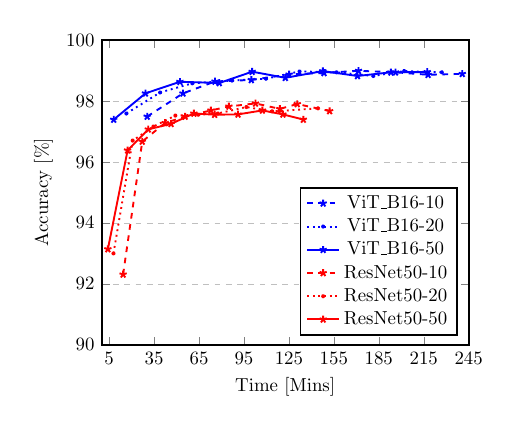
\begin{tikzpicture}[ scale=0.68]
    \begin{axis}[ xlabel={Time [Mins]},
    ylabel={Accuracy [\%]},
    xmin=0, xmax=245,
    ymin=90, ymax=100,
    xtick={5, 35, 65, 95, 125, 155, 185, 215, 245},
    ytick={90, 92, 94, 96, 98, 100},
    legend pos=south east,
    ymajorgrids=true,
    grid style=dashed,
    line width=1pt,    
    ]
\addplot[
    color=blue,
    mark=star,
    dashed
    ]
    coordinates {
    (30.38,97.49)
    (54.29,98.25)
    (75.67,98.64)
    (99.90,98.69)
    (125.13,98.87)
    (148.45,98.92)
    (171.45,98.99)
    (196.18,98.94)
    (217.94,98.86)
    (240.75,98.89)
    };
    \addlegendentry{ViT\_B16-10}

\addplot[
    color=blue,
   mark=star,
    dotted
    ]
    coordinates {
    (16.49,97.59)
    (39.01,98.28)
    (60.52,98.58)
    (87.05,98.67)
    (109.69,98.73)
    (132.09,98.97)
    (156.75,98.94)
    (181.35,98.82)
    (201.95,98.98)
    (227.10,98.94)
    };
    \addlegendentry{ViT\_B16-20}

\addplot[
    color=blue,
    mark=star,
    ]
    coordinates {
    (8.02,97.39)
    (29.24,98.25)
    (52.25,98.63)
    (78.51,98.59)
    (100.47,98.96)
    (122.60,98.76)
    (147.65,98.98)
    (170.78,98.82)
    (193.10,98.94)
    (217.38,98.95)
    };
    \addlegendentry{ViT\_B16-50}

\addplot[
    color=red,
    mark=star,
    dashed
    ]
    coordinates {
    (14.30,92.31)
    (27.07,96.67)
    (42.39,97.28)
    (55.72,97.49)
    (72.94,97.69)
    (84.95,97.82)
    (102.69,97.92)
    (118.97,97.74)
    (130.57,97.90)
    (152.17,97.67)
    };
    \addlegendentry{ResNet50-10}

\addplot[
    color=red,
    mark=star,
    dotted
    ]
    coordinates {
    (7.87,93.00)
    (20.67,96.70)
    (34.51,97.16)
    (49.19,97.52)
    (64.51,97.55)
    (77.55,97.59)
    (96.62,97.80)
    (113.80,97.66)
    (118.59,97.67)
    (144.45,97.76)
    };
    \addlegendentry{ResNet50-20}

\addplot[
    color=red,
    mark=star,
    ]
    coordinates {
    (4.13,93.14)
    (17.29,96.38)
    (31.11,97.07)
    (46.30,97.25)
    (61.54,97.59)
    (75.40,97.55)
    (91.03,97.56)
    (107.29,97.69)
    (120.97,97.56)
    (134.64,97.39)
    };
    \addlegendentry{ResNet50-50}
    \end{axis}
    \end{tikzpicture}\vspace{-1em}
\caption{Performance scores for ResNet50 and ViT\_B16 for various EDPE values and total time budgets for time, EDPE and performance on CIFAR10 (Method=CRAIG).}
\label{fig:pretrain-cf10}
\end{figure}











































 \begin{figure}
        \centering
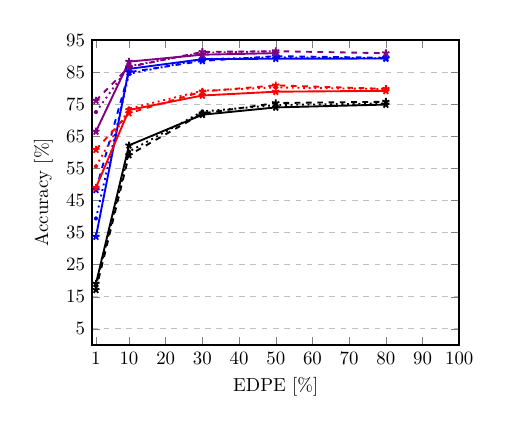
\begin{tikzpicture}[scale=0.68]
   \begin{axis}[ xlabel={EDPE [\%]},
    ylabel={Accuracy [\%]},
    xmin=0, xmax=100,
    ymin=0, ymax=95,
   xtick={1, 10, 20, 30, 40, 50, 60, 70, 80, 90, 100},
    ytick={5, 15, 25, 35, 45, 55, 65, 75, 85, 95},
    legend pos=south east,
    ymajorgrids=true,
    grid style=dashed,
    line width=1pt,
    legend style={font=\tiny}
    ]
 \addplot[
    color=blue,
    mark=star,
    dashed,
]
    coordinates {
    (1,48.30)
    (10, 84.97)
    (30,88.48)
    (50,89.97)
    (80,89.46)
    };
\label{vit10}

\addplot[
    color=blue,
    mark=star,
    dotted,
    ]
    coordinates {
    (1,39.39)
    (10, 84.46)
    (30,89.05)
    (50,89.59)
    (80,89.28)
    };
\label{vit20}

\addplot[
    color=blue,
    mark=star,
    ]
    coordinates {
    (1,33.73)
    (10, 86.00)
    (30,89.01)
    (50,89.18)
    (80,89.23)
    };
\label{vit50}

\addplot[
    color=red,
    mark=star,
    dashed,
    ]
    coordinates {
    (1,60.83)
    (10, 72.21)
    (30,78.94)
    (50,80.87)
    (80,79.76)
    };
\label{r10}

\addplot[
    color=red,
    mark=star,
    dotted,
    ]
    coordinates {
    (1,55.63)
    (10, 73.59)
    (30,79.19)
    (50,80.23)
    (80,79.70)
    };
\label{r20}

\addplot[
    color=red,
    mark=star,
    ]
    coordinates {
    (1,49.00)
    (10, 73.18)
    (30,77.71)
    (50,78.89)
    (80,79.16)
    };
\label{r50}
    

\addplot[
    color=black,
    mark=star,
    dashed,
    ]
    coordinates {
    (1,17.15)
    (10, 59.15)
    (30,72.10)
    (50,75.35)
    (80,75.76)
    };
\label{mob10}

\addplot[
    color=black,
    mark=star,
    dotted,
    ]
    coordinates {
    (1,18.36)
    (10, 60.22)
    (30,72.71)
    (50,74.73)
    (80,75.24)
    };
\label{mob20}

\addplot[
    color=black,
    mark=star,
    ]
    coordinates {
    (1,19.08)
    (10, 62.17)
    (30,71.72)
    (50,73.99)
    (80,74.88)
    };
\label{mob50}

    \addplot[
    color=violet,
    mark=star,
    dashed,
    ]
    coordinates {
    (1,76.14)
    (10, 86.60)
    (30,91.28)
    (50,91.51)
    (80,90.89)
    };
\label{s10}

\addplot[
    color=violet,
    mark=star,
    dotted,
    ]
    coordinates {
    (1,72.53)
    (10, 86.83)
    (30,91.05)
    (50,91.49)
};
\label{s20}

\addplot[
    color=violet,
    mark=star,
    ]
    coordinates {
    (1,66.49)
    (10, 88.26)
    (30,90.42)
    (50,90.90)
};
\label{s50}
    \end{axis}
    \end{tikzpicture}~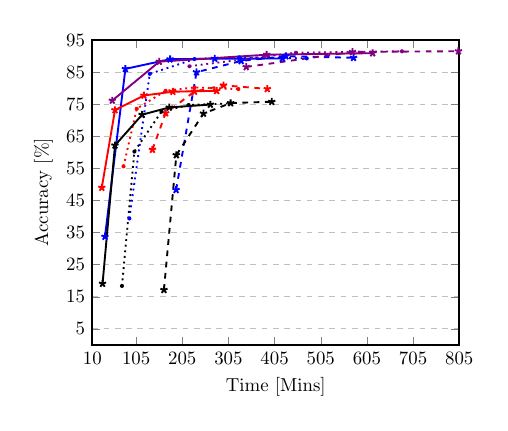
\begin{tikzpicture}[ scale=0.68]
    \begin{axis}[ xlabel={Time [Mins]},
    ylabel={Accuracy [\%]},
    xmin=10, xmax=805,
    ymin=0, ymax=95,
    xtick={10, 105, 205, 305, 405, 505, 605, 705, 805},
    ytick={5, 15, 25, 35, 45, 55, 65, 75, 85, 95},
ymajorgrids=true,
    grid style=dashed,
    line width=1pt,
]
\addplot[
    color=blue,
    mark=star,
    dashed,
]
    coordinates {
    (191.59,48.30)
    (235.84, 84.97)
    (332.62,88.48)
    (429.41,89.97)
    (575.97,89.46)
    };


\addplot[
    color=blue,
    mark=star,
    dotted,
    ]
    coordinates {
    (90.30,39.39)
    (134.54, 84.46)
    (231.33,89.05)
    (328.12,89.59)
    (474.68,89.28)
    };


\addplot[
    color=blue,
    mark=star,
    ]
    coordinates {
    (37.50,33.73)
    (81.75, 86.00)
    (178.53,89.01)
    (275.32,89.18)
    (421.88,89.23)
    };


\addplot[
    color=red,
    mark=star,
    dashed,
    ]
    coordinates {
    (140.30,60.83)
    (168.94, 72.21)
    (231.58,78.94)
    (294.23,80.87)
    (389.09,79.76)
    };


\addplot[
    color=red,
    mark=star,
    dotted,
    ]
    coordinates {
    (77.69,55.63)
    (106.33, 73.59)
    (168.98,79.19)
    (231.62,80.23)
    (326.49,79.70)
    };


\addplot[
    color=red,
    mark=star,
    ]
    coordinates {
    (30.60,49.00)
    (59.24, 73.18)
    (121.89,77.71)
    (184.53,78.89)
    (279.40,79.16)
    };


\addplot[
    color=black,
    mark=star,
    dashed,
    ]
    coordinates {
    (165.27,17.15)
    (192.15, 59.15)
    (250.97,72.10)
    (309.78,75.35)
    (398.84,75.76)
    };


\addplot[
    color=black,
    mark=star,
    dotted,
    ]
    coordinates {
    (74.34,18.36)
    (101.23, 60.22)
    (160.04,72.71)
    (218.85,74.73)
    (307.91,75.24)
    };


\addplot[
    color=black,
    mark=star,
    ]
    coordinates {
    (32.29,19.08)
    (59.18, 62.17)
    (117.99,71.72)
    (176.80,73.99)
    (265.86,74.88)
    };


    \addplot[
    color=violet,
    mark=star,
    dashed,
    ]
    coordinates {
    (343.56,86.60)
    (573.72, 91.28)
    (803.24,91.51)
};


\addplot[
    color=violet,
    mark=star,
    dotted,
    ]
    coordinates {
    (220.54,86.83)
    (451.32, 91.05)
    (680.85,91.49)
};


\addplot[
    color=violet,
    mark=star,
    ]
    coordinates {
    (53.38, 76.14)
    (155.19,88.26)
    (387.84, 90.42)
    (617.37,90.90)
};
\end{axis}
    \end{tikzpicture}\vspace{-1em}
\caption{Performance scores on TinyImagenet at SSI values of 10, 20 and 50 for pretrained CNN and transformer models (Method=CRAIG). (ViT\_B16-10 (\ref{vit10}), ViT\_B16-20 (\ref{vit20}), ViT\_B16-50 (\ref{vit50}), ResNet50-10 (\ref{r10}), ResNet50-20 (\ref{r20}), ResNet50-50 (\ref{r50}), MobileNetV3-10 (\ref{mob10}), MobileNetV3-20 (\ref{mob20}), MobileNetV3-50 (\ref{mob50}), Swin-10 (\ref{s10}), Swin-20 (\ref{s20}), and Swin-50 (\ref{s50}))}
\label{fig:pretrain-tim}
\end{figure}








































 \textbf{Data subselection under pretraining. } In this section, we investigate how pretraining (ImageNet21k) impacts model performance using coreset. Fig. \ref{fig:pretrain-cf10} shows the performance scores, and we use here CRAIG as the coreset selection method. A stable performance by both models can be seen, interestingly even when EDPE is as low as 10\% both models perform similarly. Furthermore, ViT\_B16 is consistently better than the ResNet50 model. We also see that the performance trend is consistent for  values of 10, 20 and 50. For very low EDPE values, a significant drop in the performance of the CNN models can be seen (Fig. \ref{fig:pretrain-cf10}). Overall, the stable performance for both the architectures at even very small coreset sizes as well as time budgets reveals that the pretraining on Imagenet21K serves as a very strong prior and not many samples of CIFAR10 are needed to further amplify the discriminative power of these models. 



Results on TinyImageNet classification are shown in \mbox{Fig. \ref{fig:pretrain-tim}}. We use all 4 architectures (CNN and transformer) and present scores for  values of 10, 20 and 50. It can be seen that , in general, does not impact model performance. Among the used models, the Swin transformer seems the most robust even at an EDPE value of 1\%, whereas others deteriorate significantly. However, Swin Transformer is computationally expensive. Moreover, ViT\_16 outperforms the CNN models at all coreset sizes. When compared with ResNet50, we see that at extremely low subsets, ResNet50 performs better than ViT\_B16, thus being more stable than transformers at this low extent of subset selection. Finally, we observe, when pretrained, transformer models are stable in performance across different coreset sizes.






\begin{figure}
        \centering
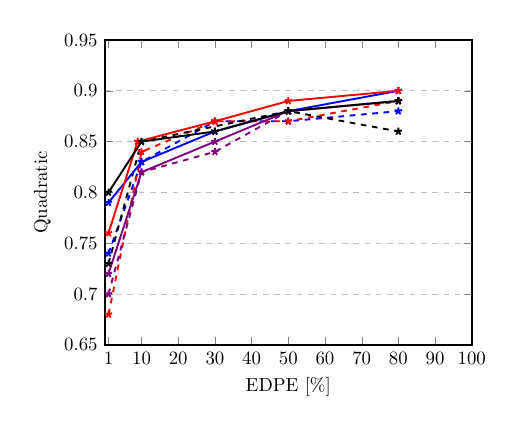
\begin{tikzpicture}[scale=0.68]
   \begin{axis}[ xlabel={EDPE [\%]},
    ylabel={Quadratic },
    xmin=0, xmax=100,
    ymin=0.65, ymax=0.95,
   xtick={1, 10, 20, 30, 40, 50, 60, 70, 80, 90, 100},
    ytick={0.65, 0.7, 0.75, 0.8, 0.85, 0.9, 0.95},
    legend pos=north east,
    ymajorgrids=true,
    grid style=dashed,
    line width=1pt,
    ]
\addplot[
    color=blue,
    mark=star,
    dashed
    ]
    coordinates {
    (1,0.74)  
    (10,0.83)  
    (30,0.87)
    (50,0.87)
    (80,0.88) 
};
\label{ViTcraig}

\addplot[
    color=red,
    mark=star,
    dashed
    ]
    coordinates {
    (1,0.68)
    (10,0.84)
    (30,0.87) 
    (50,0.87)
    (80,0.89) 
};
\label{ViTgrad}

    \addplot[
    color=violet,
    mark=star,
    dashed
    ]
    coordinates {
    (1,0.70) 
    (10,0.82)
    (30,0.84)
    (50,0.88) 
    (80,0.89)
};
\label{ViTglis}

    \addplot[
    color=black,
    mark=star,
    dashed
    ]
    coordinates {
    (1,0.73) 
    (10,0.85)
(50,0.88) 
    (80,0.86) 
};
\label{ViTrand}

    \addplot[
    color=blue,
    mark=star,
    ]
    coordinates {
    (1,0.79)
    (10,0.83) 
    (30,0.86)
    (50,0.88) 
    (80,0.90) 
};
\label{rescraig}

    \addplot[
    color=red,
    mark=star,
    ]
    coordinates {
    (1,0.76) 
    (8.92,0.85) 
    (30, 0.87)
    (50,0.89) 
    (80,0.90) 
};
\label{resgrad}

    \addplot[
    color=violet,
    mark=star,
    ]
    coordinates {
    (1,0.72) 
    (10,0.82)
    (30,0.85)
    (50,0.88) 
    (80,0.89) 


    };
\label{resglis}

    \addplot[
    color=black,
    mark=star,
    ]
    coordinates {
    (1,0.80) 
    (10,0.85) 
    (30,0.86)
    (50,0.88) 
    (80,0.89) 
};
\label{resrand}
    \end{axis}
    \end{tikzpicture}~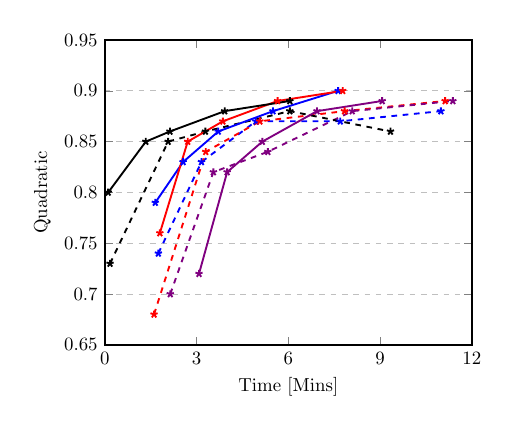
\begin{tikzpicture}[ scale=0.68]
    \begin{axis}[ xlabel={Time [Mins]},
    ylabel={Quadratic },
    xmin=0, xmax=12,
    ymin=0.65, ymax=0.95,
    xtick={0, 3, 6, 9, 12},
    ytick={0.65, 0.7, 0.75, 0.8, 0.85, 0.9, 0.95},
    legend pos=south east,
    ymajorgrids=true,
    grid style=dashed,
    line width=1pt,    
    ]
    
   \addplot[
    color=blue,
    mark=star,
    dashed
    ]
    coordinates {
    (1.75,0.74)  
    (3.16,0.83)  
    (4.94,0.87)
    (7.70,0.87)
    (10.99,0.88)
};


\addplot[
    color=red,
    mark=star,
    dashed
    ]
    coordinates {
    (1.61,0.68)
    (3.30,0.84)
    (5.07,0.87) 
    (7.84,0.88) 
    (11.13,0.89) 
};


    \addplot[
    color=violet,
    mark=star,
    dashed
    ]
    coordinates {
    (2.14,0.70) 
    (3.55,0.82)
    (5.33,0.84)
    (8.09,0.88) 
    (11.38,0.89) 
};


    \addplot[
    color=black,
    mark=star,
    dashed
    ]
    coordinates {
    (0.17,0.73) 
    (2.07,0.85)
    (3.29,0.86) 
    (6.05,0.88) 
    (9.34,0.86)
};


    \addplot[
    color=blue,
    mark=star,
    ]
    coordinates {
    (1.65,0.79)
    (2.56,0.83) 
    (3.71,0.86)
    (5.50,0.88) 
    (7.63,0.90) 
};


    \addplot[
    color=red,
    mark=star,
    ]
    coordinates {
    (1.80,0.76) 
    (2.71,0.85) 
    (3.86, 0.87) 
    (5.65,0.89) 
    (7.78,0.90) 
};
\label{resgrad}

    \addplot[
    color=violet,
    mark=star,
    ]
    coordinates {
    (3.08,0.72) 
    (4.00,0.82)
    (5.15,0.85) 
    (6.94,0.88) 
    (9.07,0.89) 


    };


    \addplot[
    color=black,
    mark=star,
    ]
    coordinates {
    (0.11,0.80) 
    (1.34,0.85) 
    (2.13,0.86) 
    (3.92,0.88)
    (6.05,0.89) 
};
\end{axis}
    \end{tikzpicture}\vspace{-1em}
\caption{Performance on APTOS-2019 classification task as a function of EDPE and total time for pretrained ResNet50 and ViT\_B16 for the 4 coreset selection methods (SSI=20). (ViT\_B16-Craig (\ref{ViTcraig}), ViT\_B16-GradMatch (\ref{ViTgrad}), ViT\_B16-GLISTER (\ref{ViTglis}), ViT\_B16-Random (\ref{ViTrand}), ResNet50-Craig (\ref{rescraig}), ResNet50-GradMatch (\ref{resgrad}), ResNet50-GLISTER (\ref{resglis}), ResNet50-Random (\ref{resrand}))}
\label{fig:ap-coresets}
\end{figure} 
\textbf{Performance on the medical dataset. } We extend our experiments to non-natural images. Fig. \ref{fig:ap-coresets}, illustrates results on the APTOS-2019 blindness detection dataset for ResNet50 and ViT\_B16. It can be seen that the ResNet50 performs better than ViT\_B16 at all coreset sizes, thereby confirming that the heavy pretraining in this case is not helping the transformers. We see that for CNN, random coreset selection is better or almost at par with GradMatch which itself performs better than the other coreset methods. For low coreset size (EDPE), random selection seems to be the most stable solution. Interestingly, when we look at the computational time, including the coreset selection time, random selection outperforms the other methods. For larger time investments, GradMatch is better than the random choice, however, for lower time budgets, random selection is the preferred choice.








\begin{figure}
        \centering
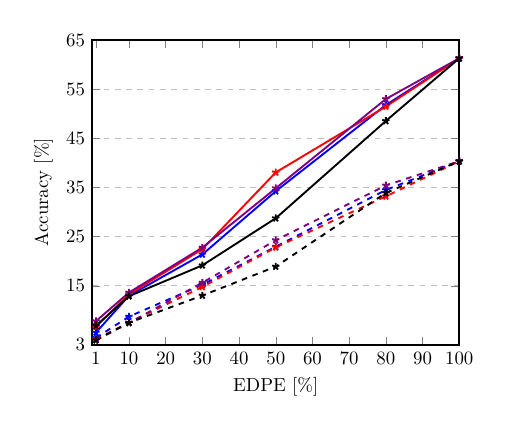
\begin{tikzpicture}[scale=0.68]
   \begin{axis}[ xlabel={EDPE [\%]},
    ylabel={Accuracy [\%]},
    xmin=0, xmax=100,
    ymin=3, ymax=65,
   xtick={1, 10, 20, 30, 40, 50, 60, 70, 80, 90, 100},
    ytick={0, 3, 15, 25, 35, 45, 55, 65},
    legend pos=north east,
    ymajorgrids=true,
    grid style=dashed,
    line width=1pt,
    ]
\addplot[
    color=blue,
    mark=star,
    dashed
    ]
    coordinates {
    (1,4.42)
    (10,8.75)
    (30,15.21)
    (50,22.96)
    (80,34.50)
    (100,40.35)
    };
\label{ViTcraig}

\addplot[
    color=red,
    mark=star,
    dashed
    ]
    coordinates {
    (1,4.14)
    (10,7.53)
    (30,14.78)
    (50,22.82)
    (80,33.21)
    (100,40.35)
    };
\label{ViTgrad}

    \addplot[
    color=violet,
    mark=star,
    dashed
    ]
    coordinates {
    (1,3.96)
    (10,7.46)
    (30,15.64)
    (50,24.28)
    (80,35.42)
    (100,40.35)
    };
\label{ViTglis}

    \addplot[
    color=black,
    mark=star,
    dashed
    ]
    coordinates {
    (1,3.96)
    (10,7.50)
    (30,13.03)
    (50,18.92)
    (80,33.89)
    (100,40.35)
    };
\label{ViTrand}

    \addplot[
    color=blue,
    mark=star,
    ]
    coordinates {
    (1,5.50)
    (10,13.00)
    (30,21.39)
    (50,34.25)
    (80,51.78)
    (100,61.28)
    };
\label{rescraig}

    \addplot[
    color=red,
    mark=star,
    ]
    coordinates {
    (1,6.67)
    (10,13.28)
    (30, 22.46)
    (50,38.07)
    (80,51.46)
    (100,61.28)
    };
\label{resgrad}

    \addplot[
    color=violet,
    mark=star,
    ]
    coordinates {
    (1,7.82)
    (10,13.64)
    (30,22.78)
    (50,34.85)
    (80,53.00) 
    (100,61.28)
    
    };
\label{resglis}

    \addplot[
    color=black,
    mark=star,
    ]
    coordinates {
    (1,6.89)
    (10,12.89)
    (30,19.17)
    (50,28.75)
    (80,48.53) 
    (100,61.28)
    };
\label{resrand}
    \end{axis}
    \end{tikzpicture}~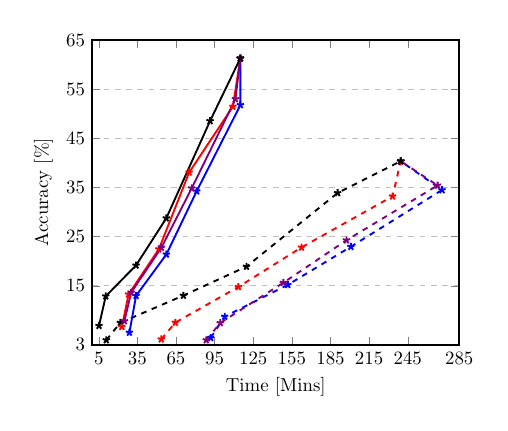
\begin{tikzpicture}[ scale=0.68]
    \begin{axis}[ xlabel={Time [Mins]},
    ylabel={Accuracy [\%]},
    xmin=0, xmax=285,
    ymin=3, ymax=65,
    xtick={5, 35, 65, 95, 125, 155, 185, 215, 245, 285},
    ytick={3, 15, 25, 35, 45, 55, 65},
    legend pos=south east,
    ymajorgrids=true,
    grid style=dashed,
    line width=1pt,    
    ]
    
    \addplot[
    color=blue,
    mark=star,
    dashed
    ]
    coordinates {
    (91.98,4.42)
    (102.86,8.75)
    (151.86,15.21)
    (200.85,22.96)
    (271.63,34.50)
    (239.53,40.35)
    };


\addplot[
    color=red,
    mark=star,
    dashed
    ]
    coordinates {
    (53.60,4.14)
    (64.49,7.53)
    (113.49,14.78)
    (162.48,22.82)
    (233.25,33.21)
    (239.53,40.35)
    };


    \addplot[
    color=violet,
    mark=star,
    dashed
    ]
    coordinates {
    (88.53,3.96)
    (99.42,7.46)
    (148.41,15.64)
    (197.41,24.28)
    (268.18,35.42)
    (239.53,40.35)
    };


    \addplot[
    color=black,
    mark=star,
    dashed
    ]
    coordinates {
    (10.88,3.96)
    (21.77,7.50)
    (70.77,13.03)
    (119.76,18.92)
    (190.53,33.89)
    (239.53,40.35)
    };


    \addplot[
    color=blue,
    mark=star,
    ]
    coordinates {
    (28.81,5.50)
    (34.03,13.00)
    (57.55,21.39)
    (81.07,34.25)
    (115.05,51.78)
    (114.99,61.28)
    };


    \addplot[
    color=red,
    mark=star,
    ]
    coordinates {
    (22.96,6.67)
    (28.19,13.28)
    (51.71, 22.46)
    (75.23,38.07)
    (109.21,51.46)
    (114.99,61.28)
    };


    \addplot[
    color=violet,
    mark=star,
    ]
    coordinates {
    (24.96,7.82)
    (30.19,13.64)
    (53.71,22.78)
    (77.23,34.85)
    (111.20,53.00) 
    (114.99,61.28)
    
    };


    \addplot[
    color=black,
    mark=star,
    ]
    coordinates {
    (5.22,6.89)
    (10.45,12.89)
    (33.97,19.17)
    (57.49,28.75)
    (91.47,48.53) 
    (114.99,61.28)
    };
\end{axis}
    \end{tikzpicture}\vspace{-1em}
\caption{Performance comparison between ImageNet-21k weight initialized \vit and ResNet50 for time, EDPE and performance on UltraMNIST with different coreset methods, SSI=20 such that ViT\_B16-Craig (\ref{ViTcraig}), ViT\_B16-GradMatch (\ref{ViTgrad}), ViT\_B16-GLISTER (\ref{ViTglis}), ViT\_B16-Random (\ref{ViTrand}), ResNet50-Craig (\ref{rescraig}), ResNet50-GradMatch (\ref{resgrad}), ResNet50-GLISTER (\ref{resglis}), ResNet50-Random (\ref{resrand})}
\label{fig:um-coresets}
\end{figure} 

\begin{figure}
        \centering
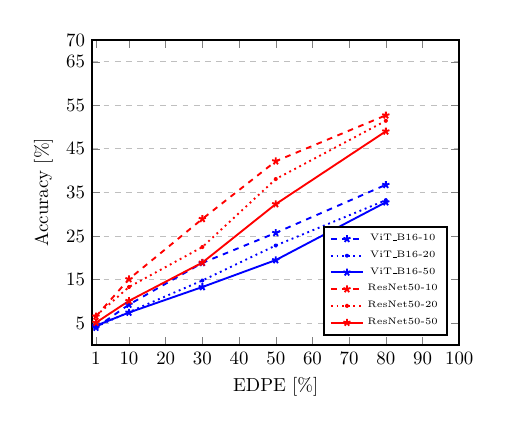
\begin{tikzpicture}[scale=0.68]
   \begin{axis}[ xlabel={EDPE [\%]},
    ylabel={Accuracy [\%]},
    xmin=0, xmax=100,
    ymin=0, ymax=70,
   xtick={1, 10, 20, 30, 40, 50, 60, 70, 80, 90, 100},
    ytick={5, 15, 25, 35, 45, 55, 65, 70},
    legend pos=south east,
    ymajorgrids=true,
    grid style=dashed,
    line width=1pt,
    legend style={font=\tiny}
    ]
 \addplot[
    color=blue,
    mark=star,
    dashed
    ]
    coordinates {
    (1,3.96)
    (10,9.25)
    (30,18.82)
    (50,25.71)
(80,36.75)
};
    \addlegendentry{ViT\_B16-10}

\addplot[
    color=blue,
   mark=star,
    dotted
    ]
    coordinates {
    (1,4.14)
    (10,7.53)
    (30,14.78)
    (50,22.82)
    (80,33.21)
    };
    \addlegendentry{ViT\_B16-20}

\addplot[
    color=blue,
    mark=star,
    ]
    coordinates {
    (1,4.39)
    (10,7.42)
    (30,13.28)
    (50,19.46)
    (80,32.75)
    };
    \addlegendentry{ViT\_B16-50}

\addplot[
    color=red,
    mark=star,
    dashed
    ]
    coordinates {
    (1,6.53)
    (10,15.10)
    (30,28.92)
    (50,42.17)
    (80,52.71)
    };
    \addlegendentry{ResNet50-10}

\addplot[
    color=red,
    mark=star,
    dotted
    ]
    coordinates {
    (1,6.67)
    (10,13.28)
    (30,22.46)
    (50,38.07)
    (80,51.46)
    };
    \addlegendentry{ResNet50-20}

\addplot[
    color=red,
    mark=star,
    ]
    coordinates {
    (1,5.10)
    (10,10.10)
    (30,18.89)
    (50,32.32)
    (80,49.03)
    };
    \addlegendentry{ResNet50-50}
    \end{axis}
    \end{tikzpicture}~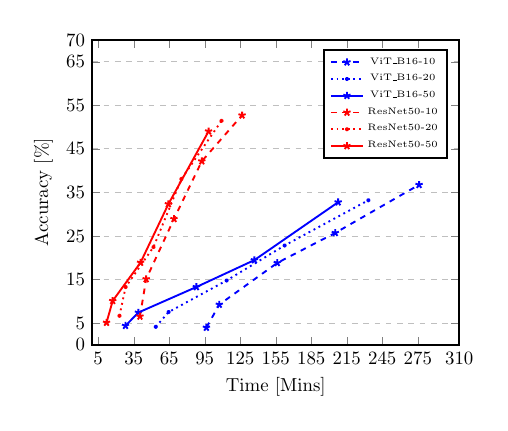
\begin{tikzpicture}[ scale=0.68]
    \begin{axis}[ xlabel={Time [Mins]},
    ylabel={Accuracy [\%]},
    xmin=0, xmax=310,
    ymin=0, ymax=70,
    xtick={5, 35, 65, 95, 125, 155, 185, 215, 245, 275, 310},
    ytick={0, 5, 15, 25, 35, 45, 55, 65, 70},
    legend pos=north east,
    ymajorgrids=true,
    grid style=dashed,
    line width=1pt,
    legend style={font=\tiny}
    ]
\addplot[
    color=blue,
    mark=star,
    dashed
    ]
    coordinates {
    (96.41,3.96)
    (107.30,9.25)
    (156.29,18.82)
    (205.29,25.71)
(276.06,36.75)
    
    };
    \addlegendentry{ViT\_B16-10}

\addplot[
    color=blue,
   mark=star,
    dotted
    ]
    coordinates {
    (53.60,4.14)
    (64.49,7.53)
    (113.49,14.78)
    (162.48,22.82)
(233.25,33.21)
    };
    \addlegendentry{ViT\_B16-20}

\addplot[
    color=blue,
    mark=star,
    ]
    coordinates {
    (28.05,4.39)
    (38.94,7.42)
    (87.94,13.28)
    (136.93,19.46)
(207.70,32.75)
    };
    \addlegendentry{ViT\_B16-50}

\addplot[
    color=red,
    mark=star,
    dashed
    ]
    coordinates {
    (40.29,6.53)
    (45.51,15.10)
    (69.03,28.92)
    (92.55,42.17)
    (126.53,52.71)
};
    \addlegendentry{ResNet50-10}

\addplot[
    color=red,
    mark=star,
    dotted
    ]
    coordinates {
    (22.96,6.67)
    (28.19,13.28)
    (51.71,22.46)
    (75.23,38.07)
    (109.21,51.46)
};
    \addlegendentry{ResNet50-20}

\addplot[
    color=red,
    mark=star,
    ]
    coordinates {
    (12.02,5.10)
    (17.24,10.10)
    (40.76,18.89)
    (64.29,32.32)
    (98.26,49.03)
};
    \addlegendentry{ResNet50-50}
    \end{axis}
    \end{tikzpicture}\vspace{-1em}
\caption{Performance comparison between pretrained ViT\_B16 and ResNet50 for time, EDPE on UltraMNIST dataset (Method=GradMatch).}
\label{fig:um-ssi}
\end{figure}
 
\begin{figure}
    \centering
    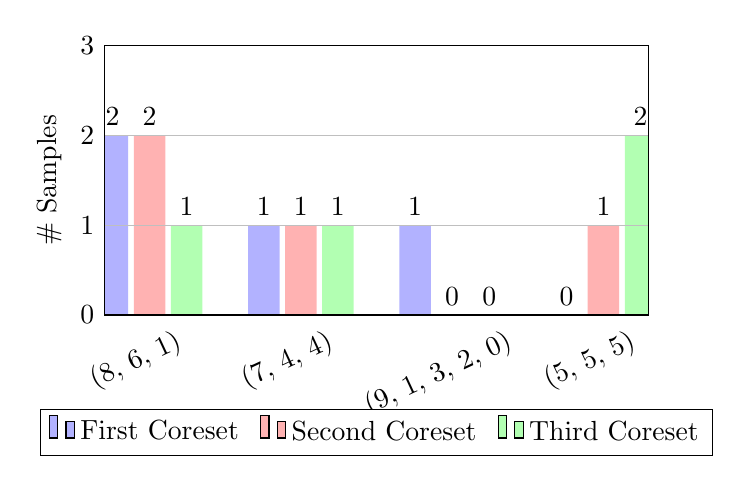
\begin{tikzpicture}[scale=1.0]
\begin{axis}[
        ybar, axis on top,
height=5cm, width=8.5cm,
        bar width=0.4cm,
        ymajorgrids, tick align=inside,
ymin=0, ymax=3,
tickwidth=0pt,
legend style={
            at={(0.5,-0.35)},
            anchor=north,
            legend columns=-1,
            /tikz/every even column/.append style={column sep=0.2cm}
        },
        ylabel={\# Samples},
        symbolic x coords={
           {(8, 6, 1)},
           {(7, 4, 4)},
           {(9, 1, 3, 2, 0)},
          {(5, 5, 5)}},
       xtick=data,
       xticklabel style={xshift=-5pt, rotate=25},
       nodes near coords={
        \pgfmathprintnumber[precision=0]{\pgfplotspointmeta}
       } 
    ]
    \addplot [draw=none, fill=blue!30] coordinates {
      ({(8, 6, 1)}, 2) 
      ({(7, 4, 4)},1) 
      ({(9, 1, 3, 2, 0)},1)
      ({(5, 5, 5)},0) 
      };
   \addplot [draw=none,fill=red!30] coordinates {
      ({(8, 6, 1)},2) 
      ({(7, 4, 4)},1) 
      ({(9, 1, 3, 2, 0)},0)
      ({(5, 5, 5)},1) 
      };
   \addplot [draw=none, fill=green!30] coordinates {
      ({(8, 6, 1)},1) 
      ({(7, 4, 4)},1) 
      ({(9, 1, 3, 2, 0)},0)
      ({(5, 5, 5)},2) 
      };

    \legend{First Coreset,Second Coreset,Third Coreset}
  \end{axis}
  \end{tikzpicture}
  \vspace{-0.8em}
    \caption{Number of samples present in different combinations of class 15 of UltraMNIST dataset in each coreset after coreset selection is done using GradMatch method.}
    \label{fig:bar-plot}
\end{figure}


 
\begin{figure*}[t]
    \centering
    \includegraphics[scale=0.11, trim=0 4.5cm 0 4.5cm, clip=true]{plots/um/samples.pdf}
    \vspace{-1em}
    \caption{UltraMNIST samples for class label 17 from the two different coresets (top and bottom) for EDPE=1\% obtained with GradMatch. Note that there is no overlap between the two coresets in terms of the combination of the digits in each image.}
    \label{fig:um-samples}
\end{figure*}

\textbf{Learning semantic coherency in non-natural images. }

We analyze here how well transformers can learn the semantic coherency of the dataset, given that the data comprises non-natural images (very different from those used in pretraining).


First, we study how the performance of the models is affected using different coreset selection methods. Fig. \ref{fig:um-coresets} presents the results for ViT\_B16 and ResNet50. We see that independent of the coreset method, the CNN model is always superior to the transformer model across all coreset sizes. This observation is consistent across the various values of SSI (Fig. \ref{fig:um-ssi}). UltraMNIST is a hard dataset to learn, and it is possible that with no similar pretraining, it is hard for transformers to learn well the desired semantic context.

In terms of the coreset size (EDPE), GradMatch outperforms the other methods while the random selection of coresets seems to perform the worst. However, in terms of the total time spent, random subset selection outperforms the other methods. This clearly indicates that although GradMatch might be a better selector of useful samples, the time spent scrutinizing the samples is not worth spending when compared to a random selection approach. For the SSI values shown in Fig. \ref{fig:um-ssi}, we see that when evaluating performance with respect to EDPE, more number of coreset selection intervals are favoured, however, when evaluating in terms of the time, lesser selection cycles are preferred. This is because the coreset selection time is significant for most methods, however, EDPE does not take that into account.

We also look at why the performance of CNNs and transformer models is extremely low when a coreset size of as low as 1\% is chosen. Our investigation reveals that this bottleneck is imposed by the fact that we conventionally choose an equal number of samples per class of the data. However, the complexity of the distribution of each class in UltraMNIST is very different. For example, class label 0 can only be formed by the combination of 3-5 occurrences of 0. However, 15 can be formed by many combinations of the digits. When selecting a coreset for this class, we tend to miss some of the combinations, thereby limiting the discriminative power of the trained model for such instances. This is also evident from the distributions shown in Fig. \ref{fig:bar-plot}. There are certain combinations of 15 that miss from one coreset to another. Clearly, the model will catastrophically forget them as soon as they are completely out of the coresets. Interestingly, this is not the worst. If the distributions of the classes are not similar, uniform sampling could lead to a situation, where the distribution of the hard class could change completely between two coresets. Fig. \ref{fig:um-samples} shows the training samples of class 17 from two different coresets of EDPE = 1\%. As can be seen, the two sets are completely different which implies that it would be hard for the model to generalize for this class for very small coreset sizes. Overall, the takeaway is that the complexity of the distribution per class should be taken into consideration when constructing the coresets.

\subsection{Discussion}
In this section, we summarize the insights from experiments and present answers to some intriguing questions.


\textit{Should random coreset selection be a preferred choice? }Our results reveal that when comparing performance in terms of time budget, the random selection of the coresets is a more time-efficient choice than the other coreset selection methods. Clearly, one of the factors in favour of random selection is that the coreset selection time is almost zero. From a practical point of view, the impact of the small gains observed by other coreset selection methods would be diminished if the associated subset selection time is significant. Thus, unless the coreset method is very efficient or parallelizable to the extent that the selection time can be made very small, random coreset selection should be a preferred choice for training models in a data-efficient manner.

\textit{Choosing the right subset selection interval (SSI). }There is no right SSI value, but one could optimize this choice based on the available resources. It is evident that when measured purely in terms of EDPE, coreset selection methods perform better than a random choice, and it can be expected that the more the selection frequency, the better the model performance. However, so far, we have seen that the computational time associated with coreset selection is not negligible, and as long as the overall time is below the desired threshold, the choice of SSI is good.



\textit{Should coresets be chosen uniformly across the classes?}
We argue that when constructing the coresets, methods should also focus on constructing the approximate distribution of every class. This would require sampling more samples from the class that is more complex while sparse sampling from the easier one. This way, the small coreset budget could be used in a more appropriate. While this could raise the challenges of class imbalance among others, we still believe that coresets should not be chosen uniformly across the classes, but in a more adaptive manner.




